\chapter{Le funzioni armoniche}
\label{chap:funzioni_armoniche}

Ogni accordo all'interno di una tonalità non è semplicemente un insieme di note sovrapposte: possiede una \textbf{funzione armonica}, ovvero un ruolo specifico nel discorso musicale. Comprendere le funzioni armoniche significa comprendere la logica interna del sistema tonale, le forze di attrazione e repulsione che governano il movimento da un accordo all'altro.

\section{Le tre funzioni fondamentali}
\label{sec:tre_funzioni}

Nel sistema tonale, tutti gli accordi possono essere ricondotti a tre funzioni principali: \textbf{tonica}, \textbf{dominante} e \textbf{sottodominante}. Queste funzioni rappresentano rispettivamente riposo, tensione e movimento.

\begin{esempio}[Funzioni fondamentali]
\musica{es_cap05_01}
\end{esempio}

\begin{definizione}[Funzioni armoniche]
	
	\begin{itemize}
		\item \label{def:funzione_tonica}
		La \textbf{funzione di tonica} rappresenta il punto di riposo, la stabilità, la "casa" della tonalità. L'accordo principale che svolge questa funzione è la \textbf{triade sul I grado}. La tonica è il punto di partenza e di arrivo della maggior parte dei discorsi armonici.
		\item \label{def:funzione_dominante}
		La \textbf{funzione di dominante} rappresenta la massima tensione armonica, l'impulso irresistibile verso la risoluzione sulla tonica. L'accordo principale che svolge questa funzione è la \textbf{triade sul V grado}. La dominante contiene la \textit{sensibile} (VII grado della scala), che tende con forza verso la tonica.
		\item 	\label{def:funzione_sottodominante}
		La \textbf{funzione di sottodominante} rappresenta il movimento, l'allontanamento dalla tonica, la preparazione della dominante. L'accordo principale che svolge questa funzione è la \textbf{triade sul IV grado}. La sottodominante contiene il IV grado della scala, che tende a scendere verso il III grado.
	\end{itemize}
\end{definizione}

	La progressione, ovvero successione di accordi, I - IV - V - I rappresenta il modello base del movimento armonico tonale: partenza dalla tonica, allontanamento attraverso la sottodominante, tensione sulla dominante, ritorno alla tonica.

\section{Gli accordi secondari e le loro funzioni}
\label{sec:accordi_secondari}

Gli accordi costruiti sui gradi II, III, VI e VII, pur avendo una loro identità, possono essere pensati come "sostituti" delle tre funzioni principali. La chiave per capire questa relazione sta nelle \textbf{note comuni} che questi accordi condividono con gli accordi principali.

\begin{esempio}[II come sottodominante]
\musica{es_cap05_02}
\end{esempio}

Due accordi che condividono molte note tendono a svolgere funzioni simili. Osserviamo le triadi diatoniche di Do maggiore, che useremo per comprendere le prossime definizioni:

\begin{center}
\begin{tabular}{|c|c|c|c|c|}
\hline
\textbf{Grado} & \textbf{Note} & \textbf{Note comuni con I} & \textbf{Note comuni con IV} & \textbf{Note comuni con V} \\
\hline
I & Do Mi Sol & --- & Do & Sol \\
II & Re Fa La & --- & Fa La & Re \\
III & Mi Sol Si & Mi Sol & --- & Sol Si \\
IV & Fa La Do & Do & --- & --- \\
V & Sol Si Re & Sol & --- & --- \\
VI & La Do Mi & Do Mi & La & --- \\
VII & Si Re Fa & --- & Fa & Si Re \\
\hline
\end{tabular}
\end{center}

\subsection{Accordi in ogni grado della scala}
\label{subsec:accordi_funzioni}

\begin{definizione}[Accordi con funzione di tonica]
	\label{def:accordi_tonica}
	Oltre al I grado, possono svolgere funzione di tonica:
	\begin{itemize}
		\item \textbf{III grado:} condivide due note con la tonica. È la tonica "debole" o "relativa".
		\item \textbf{VI grado:} condivide due note con la tonica. È frequentemente usato nella \textit{cadenza d'inganno} come sostituto della tonica.
	\end{itemize}
\end{definizione}


\begin{definizione}[Accordi con funzione di sottodominante]
	\label{def:accordi_sottodominante}
	Oltre al IV grado, possono svolgere funzione di sottodominante:
	\begin{itemize}
		\item \textbf{II grado:} condivide due note con la sottodominante. È un sostituto molto comune del IV grado, specialmente nella progressione II - V - I.
		\item \textbf{VI grado:} condivide una nota con la sottodominante. In certi contesti può avere sfumatura sottodominante.
	\end{itemize}
\end{definizione}


\begin{definizione}[Accordi con funzione di dominante]
	\label{def:accordi_dominante}
	Oltre al V grado, può svolgere funzione di dominante:
	\begin{itemize}
		\item \textbf{VII grado:} condivide due note con la dominante e, soprattutto, contiene la sensibile. È essenzialmente una dominante senza fondamentale.
	\end{itemize}
\end{definizione}

\begin{matematica}[L'identità del III grado: tra Tonica e Dominante]
	Possiamo analizzare la parentela tra gli accordi utilizzando la teoria degli insiemi. Considerando le triadi in Do maggiore come insiemi di note, osserviamo:
	\begin{itemize}
		\item $I = \{Do, Mi, Sol\}$
		\item $III = \{Mi, Sol, Si\}$
		\item $V = \{Sol, Si, Re\}$
	\end{itemize}
	Si nota che la cardinalità dell'intersezione è identica in entrambi i casi: 
	$|I \cap III| = 2$ ($Mi, Sol$) e $|V \cap III| = 2$ ($Sol, Si$). 
	
	Perché allora il III grado è considerato una "tonica debole"  invece di una dominante? La risposta risiede nella \textbf{gerarchia pesata} degli elementi:
	\begin{enumerate}
		\item Il $Mi$ è la \textit{caratteristica modale} della tonica; la sua presenza nel III grado stabilisce un legame identitario fortissimo con la "casa" della tonalità.
		\item Sebbene il III grado contenga la sensibile ($Si$), manca della \textit{fondamentale} della dominante ($Sol$ al basso o come nota portante), che è necessaria per generare la spinta propulsiva verso la risoluzione.
	\end{enumerate}
	Pertanto, pur avendo lo stesso numero di note in comune con il V grado, la "forza gravitazionale" esercitata dalle note in comune con il I grado prevale, rendendolo un sostituto del riposo piuttosto che della tensione.
\end{matematica}


	Il seguente schema riassume le relazioni funzionali nel modo maggiore:
	
	\begin{center}
	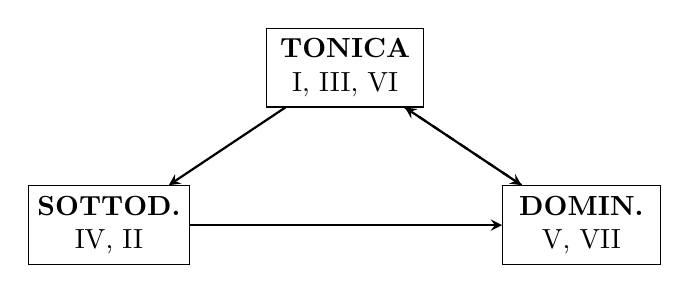
\begin{tikzpicture}[
		box/.style={draw, minimum width=2cm, minimum height=1cm, align=center},
		arrow/.style={->, >=stealth, thick}
	]
	% Tonica
	\node[box, fill=white] (T) at (0,0) {\textbf{TONICA}\\I, III, VI};
	% Sottodominante  
	\node[box, fill=white] (S) at (-3,-2) {\textbf{SOTTOD.}\\IV, II};
	% Dominante
	\node[box, fill=white] (D) at (3,-2) {\textbf{DOMIN.}\\V, VII};
	
	% Frecce
	\draw[arrow] (T) -- (S);
	\draw[arrow] (S) -- (D);
	\draw[arrow] (D) -- (T);
	\draw[arrow, dashed] (T) -- (D);
	\end{tikzpicture}
	\end{center}
	
	Il percorso tipico è T → S → D → T, ma è possibile anche il collegamento diretto T → D → T.


\section{L'armonizzazione della scala: la regola dell'ottava}
\label{sec:regola_ottava_funzioni}

La \textbf{Regola dell'Ottava} è uno schema pratico e sistematico che insegna come armonizzare ogni grado della scala quando esso appare al basso. Questa regola, che ha origini storiche nella pratica del basso continuo del periodo barocco, rappresenta un potente strumento didattico per comprendere la logica dell'armonizzazione.

\begin{definizione}[Regola dell'ottava]
	\label{def:versioni_regola_ottava}
	Nel corso di questo manuale presenteremo la Regola dell'Ottava in \textbf{tre versioni progressive}, ciascuna più "completa" e "ricca" della precedente:
	
	\begin{enumerate}
		\item \textbf{Versione preliminare (questo capitolo):} utilizza esclusivamente \textbf{triadi} in stato fondamentale e rivolti.
		\item \textbf{Versione intermedia (Capitolo \ref{chap:settima_dominante}):} integra le \textbf{settime di dominante} e i loro rivolti nello schema.
		\item \textbf{Versione completa (Capitolo successivo):} include l'intero arsenale delle settime per una realizzazione più ricca e flessibile.
	\end{enumerate}
	
	Questo approccio progressivo permette di padroneggiare gradualmente la complessità della regola, evitando di essere sopraffatti dalle numerose possibilità armoniche fin dall'inizio.
\end{definizione}

\subsection{Movimenti del basso e assegnazione delle funzioni}
\label{subsec:principio_regola_ottava}

Quando il basso si muove per grado congiunto, la scelta dell'accordo dipende dalla posizione della nota all'interno della scala. Il principio guida di questa versione preliminare è quello di utilizzare i rivolti per mantenere il movimento melodico senza appesantire la struttura con troppi stati fondamentali.

\begin{regola}{Regola dell'Ottava (triadi) - Scala Maggiore Ascendente}
	\label{reg:regola_ottava_maggiore_asc}
	Armonizzazione dei gradi della scala maggiore in movimento ascendente:
	
	\begin{itemize}
		\item \textbf{I grado:} Accordo di \textbf{I} in stato fondamentale (5)
		\item \textbf{II grado:} Accordo di \textbf{VII} in primo rivolto (6)
		\item \textbf{III grado:} Accordo di \textbf{I} in primo rivolto (6)
		\item \textbf{IV grado:} Accordo di \textbf{II} in primo rivolto (6)
		\item \textbf{V grado:} Accordo di \textbf{V} in stato fondamentale (5) — oppure I$^6_4$ di passaggio
		\item \textbf{VI grado:} Accordo di \textbf{IV} in primo rivolto (6)
		\item \textbf{VII grado:} Accordo di \textbf{V} in primo rivolto (6)
		\item \textbf{VIII grado:} Accordo di \textbf{I} in stato fondamentale (5)
	\end{itemize}
\end{regola}



\begin{regola}{Regola dell'Ottava (triadi) - Scala Maggiore Discendente}
	\label{reg:regola_ottava_maggiore_disc}
	Armonizzazione dei gradi della scala maggiore in movimento discendente:
	
	\begin{itemize}
		\item \textbf{VIII grado:} Accordo di \textbf{I} in stato fondamentale (5)
		\item \textbf{VII grado:} Accordo di \textbf{V} in primo rivolto (6)
		\item \textbf{VI grado:} Accordo di \textbf{IV} in primo rivolto (6)
		\item \textbf{V grado:} Accordo di \textbf{V} in stato fondamentale (5)
		\item \textbf{IV grado:} Accordo di \textbf{II} in primo rivolto (6)
		\item \textbf{III grado:} Accordo di \textbf{I} in primo rivolto (6)
		\item \textbf{II grado:} Accordo di \textbf{VII} in primo rivolto (6)
		\item \textbf{I grado:} Accordo di \textbf{I} in stato fondamentale (5)
	\end{itemize}
\end{regola}



\begin{regola}{Regola dell'Ottava (triadi) - Scala Minore Armonica Ascendente}
	\label{reg:regola_ottava_minore_asc}
	Armonizzazione dei gradi della scala minore armonica in movimento ascendente:
	
	\begin{itemize}
		\item \textbf{I grado:} Accordo di \textbf{I} in stato fondamentale (5)
		\item \textbf{II grado:} Accordo di \textbf{VII°} in primo rivolto (6)
		\item \textbf{III grado:} Accordo di \textbf{I} in primo rivolto (6)
		\item \textbf{IV grado:} Accordo di \textbf{II°} in primo rivolto (6)
		\item \textbf{V grado:} Accordo di \textbf{V} in stato fondamentale (5) — oppure I$^6_4$ di passaggio
		\item \textbf{VI grado:} Accordo di \textbf{IV} in primo rivolto (6)
		\item \textbf{VII grado:} Accordo di \textbf{V} in primo rivolto (6)
		\item \textbf{VIII grado:} Accordo di \textbf{I} in stato fondamentale (5)
	\end{itemize}
\end{regola}



\begin{regola}{Regola dell'Ottava (triadi) - Scala Minore Armonica Discendente}
	\label{reg:regola_ottava_minore_disc}
	Armonizzazione dei gradi della scala minore armonica in movimento discendente:
	
	\begin{itemize}
		\item \textbf{VIII grado:} Accordo di \textbf{I} in stato fondamentale (5)
		\item \textbf{VII grado:} Accordo di \textbf{V} in primo rivolto (6) — può essere \textbf{III}
		\item \textbf{VI grado:} Accordo di \textbf{IV} in primo rivolto (6)
		\item \textbf{V grado:} Accordo di \textbf{V} in stato fondamentale (5)
		\item \textbf{IV grado:} Accordo di \textbf{II°} in primo rivolto (6)
		\item \textbf{III grado:} Accordo di \textbf{I} in primo rivolto (6)
		\item \textbf{II grado:} Accordo di \textbf{VII°} in primo rivolto (6)
		\item \textbf{I grado:} Accordo di \textbf{I} in stato fondamentale (5)
	\end{itemize}
\end{regola}



\begin{regola}{Regola dell'Ottava (triadi) - Scala Minore Melodica Ascendente}
	\label{reg:regola_ottava_melodica_asc}
	Armonizzazione dei gradi della scala minore melodica in movimento ascendente (con VI e VII gradi alterati):
	
	\begin{itemize}
		\item \textbf{I grado:} Accordo di \textbf{I} in stato fondamentale (5)
		\item \textbf{II grado:} Accordo di \textbf{VII°} in primo rivolto (6)
		\item \textbf{III grado:} Accordo di \textbf{I} in primo rivolto (6)
		\item \textbf{IV grado:} Accordo di \textbf{II} in primo rivolto (6)
		\item \textbf{V grado:} Accordo di \textbf{V} in stato fondamentale (5) — oppure I$^6_4$ di passaggio
		\item \textbf{VI grado:} Accordo di \textbf{IV} in primo rivolto (6)
		\item \textbf{VII grado:} Accordo di \textbf{V} in primo rivolto (6)
		\item \textbf{VIII grado:} Accordo di \textbf{I} in stato fondamentale (5)
	\end{itemize}
	
	\textit{Nota: Nella scala minore melodica ascendente, il VI e VII grado sono alterati ascendentemente, rendendo il IV grado maggiore (II) e il VII grado maggiore (VII), come nella scala maggiore.}
\end{regola}


\begin{regola}{Regola dell'Ottava (triadi) - Scala Minore Melodica Discendente}
	\label{reg:regola_ottava_melodica_disc}
	Armonizzazione dei gradi della scala minore melodica in movimento discendente (forma naturale):
	
	\begin{itemize}
		\item \textbf{VIII grado:} Accordo di \textbf{I} in stato fondamentale (5)
		\item \textbf{VII grado:} Accordo di \textbf{III} in primo rivolto (6) — oppure \textbf{V}$^6$
		\item \textbf{VI grado:} Accordo di \textbf{IV} in primo rivolto (6)
		\item \textbf{V grado:} Accordo di \textbf{V} in stato fondamentale (5)
		\item \textbf{IV grado:} Accordo di \textbf{II°} in primo rivolto (6)
		\item \textbf{III grado:} Accordo di \textbf{I} in primo rivolto (6)
		\item \textbf{II grado:} Accordo di \textbf{VII°} in primo rivolto (6)
		\item \textbf{I grado:} Accordo di \textbf{I} in stato fondamentale (5)
	\end{itemize}
	
	\textit{Nota: Nella scala minore melodica discendente si utilizzano i gradi naturali (VI e VII abbassati), coincidendo con la scala minore naturale.}
\end{regola}


\section{Basso che salta o che procede per grado congiunto}
\label{sec:basso_salti_gradi}

La distinzione tra movimento melodico (grado congiunto) e movimento armonico (salto) è fondamentale per decidere quale stato dell'accordo utilizzare.

\begin{regola}[Scelta dello stato dell'accordo in base al movimento del basso]
	\label{reg:stato_basso}
	\begin{itemize}
		\item \textbf{Basso per grado congiunto}: si applica la \textbf{Regola dell'Ottava}.
		\item \textbf{Basso che salta}: si predilige lo \textbf{stato fondamentale}, poiché il salto indica un cambio di pilastro armonico.
		\item \textbf{Eccezione del V grado}: l'accordo di dominante può essere sempre usato in stato fondamentale per sottolineare la forza delle cadenze, indipendentemente dal movimento del basso.
	\end{itemize}
\end{regola}

\begin{regola}[Salto d'ottava al basso]
	\label{reg:salto_ottava_basso}
	Quando il basso compie un salto d'ottava (sia verso l'alto che verso il basso), la seconda nota del salto si numera generalmente con il \textbf{6} (primo rivolto della triade), creando un arpeggio armonico più fluido e variato.
\end{regola}



\section{Il secondo rivolto e la funzione del V grado}
\label{sec:secondo_rivolto_regola}

In questa versione preliminare della regola, l'accordo sul \textbf{V grado} della scala ammette una duplice natura. Sebbene la triade di dominante in stato fondamentale sia la scelta più comune per garantire stabilità, è possibile utilizzare il secondo rivolto della tonica (\textbf{I6/4}).

L'uso del I6/4 sul quinto grado della scala può avvenire in due modalità:

\begin{itemize}
	\item \textbf{I6/4 di passaggio}: quando il basso tocca il V grado muovendosi tra il IV e il VI (o viceversa), creando un collegamento morbido.
	\item \textbf{I6/4 cadenzale}: quando il V grado al basso viene "appoggiato" da quarta e sesta che poi risolvono sulla terza e quinta dell'accordo di dominante (V). Questo uso sarà approfondito nei capitoli successivi.
\end{itemize}

Queste opzioni rendono il V grado della scala uno dei punti più flessibili e interessanti dell'intera Regola dell'Ottava, permettendo al compositore di scegliere tra la forza della dominante pura e l'eleganza della sospensione cadenzale.

\begin{fisica}[Perché il I6/4 sul V grado suona "sospeso"?]
	Quando suoniamo il secondo rivolto della tonica (I6/4) con il Sol al basso (V grado in Do maggiore), le note sono Sol-Do-Mi. Dal punto di vista acustico, questo accordo presenta una caratteristica particolare:
	
	\begin{itemize}
		\item La quarta Sol-Do crea un intervallo il cui rapporto di frequenza è 4:3
		\item Questo rapporto non appare tra i primi armonici semplici della nota al basso (Sol)
		\item Gli armonici di Sol includono: Sol, Re, Sol, Si, Re... ma non Do
		\item Il Do risulta quindi "alieno" rispetto alla serie armonica naturale del basso
	\end{itemize}
	
	Questa "estraneità acustica" del Do rispetto al basso Sol genera la sensazione di instabilità e sospensione che caratterizza il I6/4. Quando questo accordo risolve sul V (Sol-Si-Re-Fa), la quarta Sol-Do scende alla terza Sol-Si, che è invece presente come terzo armonico del basso, creando una risoluzione acusticamente "naturale" e soddisfacente.
	
	Questa è la ragione fisica per cui il secondo rivolto, pur essendo tecnicamente un accordo di tonica, funziona armonicamente come preparazione della dominante: la serie armonica stessa ci guida verso la risoluzione.
\end{fisica}

% ============================================================
% CAPITOLO 4
% ============================================================
